\documentclass[12pt, titlepage]{article}

\usepackage{fullpage}
\usepackage[round]{natbib}
\usepackage{multirow}
\usepackage{booktabs}
\usepackage{tabularx}
\usepackage{graphicx}
\usepackage{float}
\usepackage{hyperref}
\hypersetup{ colorlinks, citecolor=blue, filecolor=black, linkcolor=red,
    urlcolor=blue }

%% Comments

\usepackage{color}

\newif\ifcomments\commentsfalse %displays comments
%\newif\ifcomments\commentsfalse %so that comments do not display

\ifcomments
\newcommand{\authornote}[3]{\textcolor{#1}{[#3 ---#2]}}
\newcommand{\todo}[1]{\textcolor{red}{[TODO: #1]}}
\else
\newcommand{\authornote}[3]{}
\newcommand{\todo}[1]{}
\fi

\newcommand{\wss}[1]{\authornote{blue}{SS}{#1}} 
\newcommand{\plt}[1]{\authornote{magenta}{TPLT}{#1}} %For explanation of the template
\newcommand{\an}[1]{\authornote{cyan}{Author}{#1}}

%% Common Parts

\newcommand{\progname}{ProgName} % PUT YOUR PROGRAM NAME HERE
\newcommand{\authname}{Team \#, Team Name
\\ Student 1 name
\\ Student 2 name
\\ Student 3 name
\\ Student 4 name} % AUTHOR NAMES                  

\usepackage{hyperref}
    \hypersetup{colorlinks=true, linkcolor=blue, citecolor=blue, filecolor=blue,
                urlcolor=blue, unicode=false}
    \urlstyle{same}
                                


\newcounter{acnum}
\newcommand{\actheacnum}{AC\theacnum}
\newcommand{\acref}[1]{AC\ref{#1}}

\newcounter{ucnum}
\newcommand{\uctheucnum}{UC\theucnum}
\newcommand{\uref}[1]{UC\ref{#1}}

\newcounter{mnum}
\newcommand{\mthemnum}{M\themnum}
\newcommand{\mref}[1]{M\ref{#1}}

\begin{document}

\title{System Design for \progname{}} 
\author{\authname}
\date{\today}

\maketitle

\pagenumbering{roman}

\section{Revision History}

\begin{tabularx}{\textwidth}{p{3cm}p{2cm}X} \toprule {\bf Date} & {\bf Version}
& {\bf Notes}\\
\midrule
Jan 18, 2023 & 1.0 & Revision 0\\
\bottomrule
\end{tabularx}

\newpage

\section{Reference Material}

This section records information for easy reference.

\subsection{Abbreviations and Acronyms}

See SRS Documentation at
\href{https://github.com/parkd-app/park-d/blob/main/docs/SRS/SRS.pdf}{Park'd
Software Requirements Specification}.\\

\noindent
\renewcommand{\arraystretch}{1.2}
\begin{tabular}{l l} 
  \toprule		
  \textbf{Symbol} & \textbf{Description}\\
  \midrule 
  \progname & Parking Lot Application\\
  \bottomrule
\end{tabular}\\

\newpage

\tableofcontents

\newpage

\listoftables

\listoffigures

\newpage

\pagenumbering{arabic}

\section{Introduction}

This System Design document provides an overview of the design of the Park'd
system. A detailed specification and guide of the system modules can be found in
the
\href{https://github.com/parkd-app/park-d/tree/main/docs/Design/MIS/MIS.pdf}{Module
Interface Specification} and
\href{https://github.com/parkd-app/park-d/tree/main/docs/Design/MG/MG.pdf}{Module
Guide} documents, respectively.

\section{Purpose}

The purpose of our system is provide a way for users to identify available
parking spaces and reserve said spaces prior to arriving at the parking space,
thereby reducing frustration. The system also provides instructions for the user
to navigate to their desired parking space. In addition, the administrator for
the parking space has the ability to modify certain elements of the parking
space, such as the layout and which parking spaces are reserved.

The purpose of this design documentation is to identify the overall system
components of our project, their behaviours, and how they will work with one
another to comprise the project as a whole. Furthermore, we will use this report
to discuss how error handling will be implemented to account for undesired
behaviours.

\section{Scope}

The system is meant to direct drivers to open parking spots. The driver will
provide their location and a layout of their parking lot is displayed. Drivers
will select an open spot and follow directions to it.

\begin{figure}[ht]
    \begin{center}
        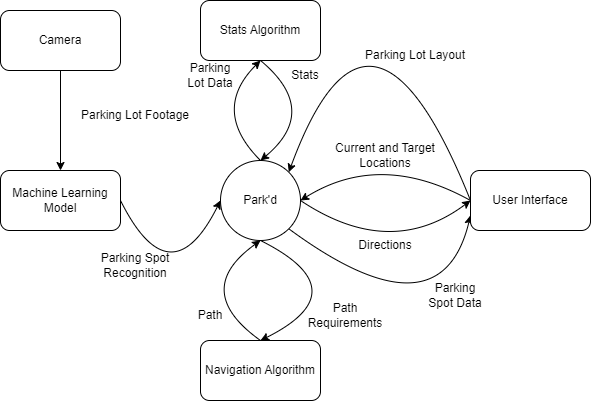
\includegraphics[scale=0.5]{ContextDiagram.png}
        \caption{Context Diagram}
    \end{center}
\end{figure}

\newpage

\section{Project Overview}

The following section is to outline the normal behavior of Park'd and undesired
event handling.

\subsection{Normal Behaviour}

Normal behaviour entails regular users being able to sign in, so that parking
lots that are shown to them are tailored specifically to their profile, which
consists of their vehicle type and their parking preference (regular or
accessibility). Afterwards, users can select available parking spaces and then
receive instructions to arrive at the selected parking space. 

For administrators, the experience involves the ability to modify the layout of
the parking space and designating certain parking spaces as either reserved or
accessibility parking.

\subsection{Undesired Event Handling}

For the normal behaviour described above, there are many points of failure,
which can result in undesired events. For example, the user may not be able to
log in due to database connection issue. In this case, we would allow the user
to still use the application, but the parking spaces shown to them may not be
necessarily tailored to their needs. Another example is when the parking
directions that are provided for a specified parking space are blocked by
obstacles. To prevent this issue, there will be multiple algorithms that all
compute the parking directions using different techniques.

In general, undesired events will be handled using multiple algorithms, which
build upon the redundancy principle, or by using software that will still
function if back-end features do not work correctly.


\newpage
\subsection{Component Diagram}
The following is a component diagram of the Park'd system.

\begin{figure}[ht]
    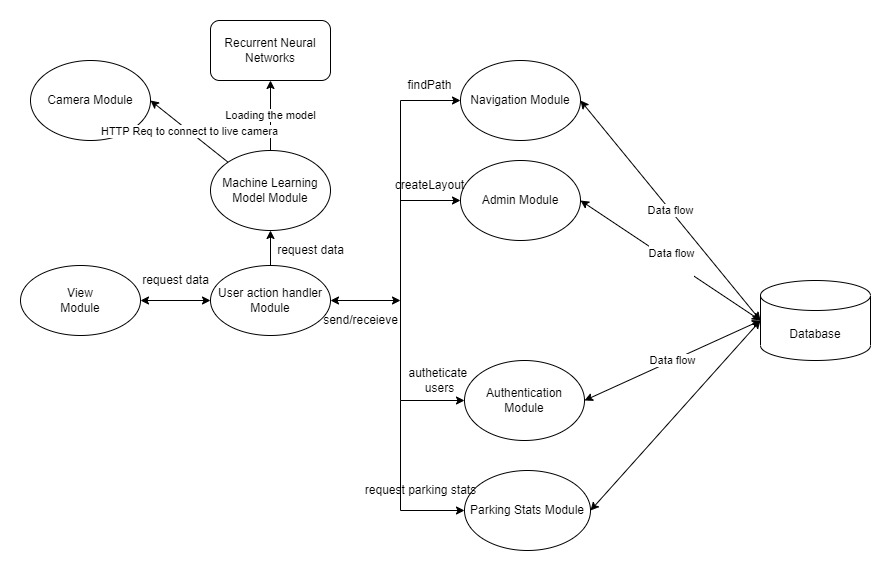
\includegraphics[scale=0.55]{component.jpg}
    \caption{Component Diagram}
\end{figure}


\newpage
\subsection{Connection Between Requirements and Design} \label{SecConnection}
The following table is to document decisions that are made between the
requirements and the design.

\begin{table}[h!]
\caption{Design Decisions and Requirements}
    \centering
    \begin{tabular}{|p{10cm}|c|}
    \hline
    \textbf{Design Decision} & \textbf{Requirements} \\
    \hline
    The software sends a prompt asking for users' current location information
    in order to use it for navigation & FR1, FR2 \\
    \hline
    A sign-up function will be considered in future revisions as currently,
    there are privacy and security concerns regarding sensitive information
    being leaked out & FR1, FR2\\
    \hline
    Admin console is created to allow parking lot administrator to recreate the
    parking lot layout and thus provide information for users later when they
    are looking for parking spaces & FR5, FR6, FR7\\
    \hline
    Mapping API is used to display routing information as clearly as possible to
    the user & FR11, FR13\\
    \hline
    The time interval between every update of the parking lot state and display
    must be short & FR17, FR18, FR20\\
    \hline
    The information of the parking lot provided to user should also be available
    to the parking lot admin & FR26, FR27, FR28, FR29\\
    \hline
    \end{tabular}
\end{table}

\section{System Variables}

This section is not applicable to software engineering projects.

\subsection{Monitored Variables}
N/A

\subsection{Controlled Variables}
N/A

\subsection{Constants Variables}
N/A

\section{User Interfaces} 

\href{https://www.figma.com/file/LglAu6OBHHntlaihSaGUhv/DESIGN-DRAFT?node-id=0%3A1&t=lYDORXYJa3TJiJ7X-1}{Figma}
was used to prototype the user interface. The user interface consists of three
different parts - Login Screen, User View, and Admin View.

For the Login Screen, the design allows both parking lot managers and users to
login to an account on the system and prompts them to provide the appropriate
information to do so (Figure \ref{fig:login}).

With the User View, users are able to see parking lots nearby and their
availability, select/search for a parking lot, select a parking spot to navigate
to, as well as change settings and preferences (Figure \ref{fig:youarehere},
Figure \ref{fig:description}, Figure \ref{fig:pickspot}, Figure
\ref{fig:settings}).

Lastly, for the Admin View, admins are also able to see the analytics of their
parking lot including how many available parking spaces there are, the division
of parking spaces based on specialty spaces, as well as make edits to the
parking lots they own (Figure \ref{fig:analytics}, Figure \ref{fig:edit}). The
Admin View also includes settings similar to that of the User View.

\section{Design of Hardware}

This section is not applicable to the Park'd project.

\section{Design of Electrical Components}

This section is not applicable to the Park'd project.

\section{Design of Communication Protocols}

This section is not applicable to the Park'd project.

\newpage
\section{Timeline}

A timeline of tasks and responsibilities leading up to the Revision 0
Demonstration can be found in Figure \ref{fig:timeline} below.

\begin{figure}[h]
    \begin{center}
        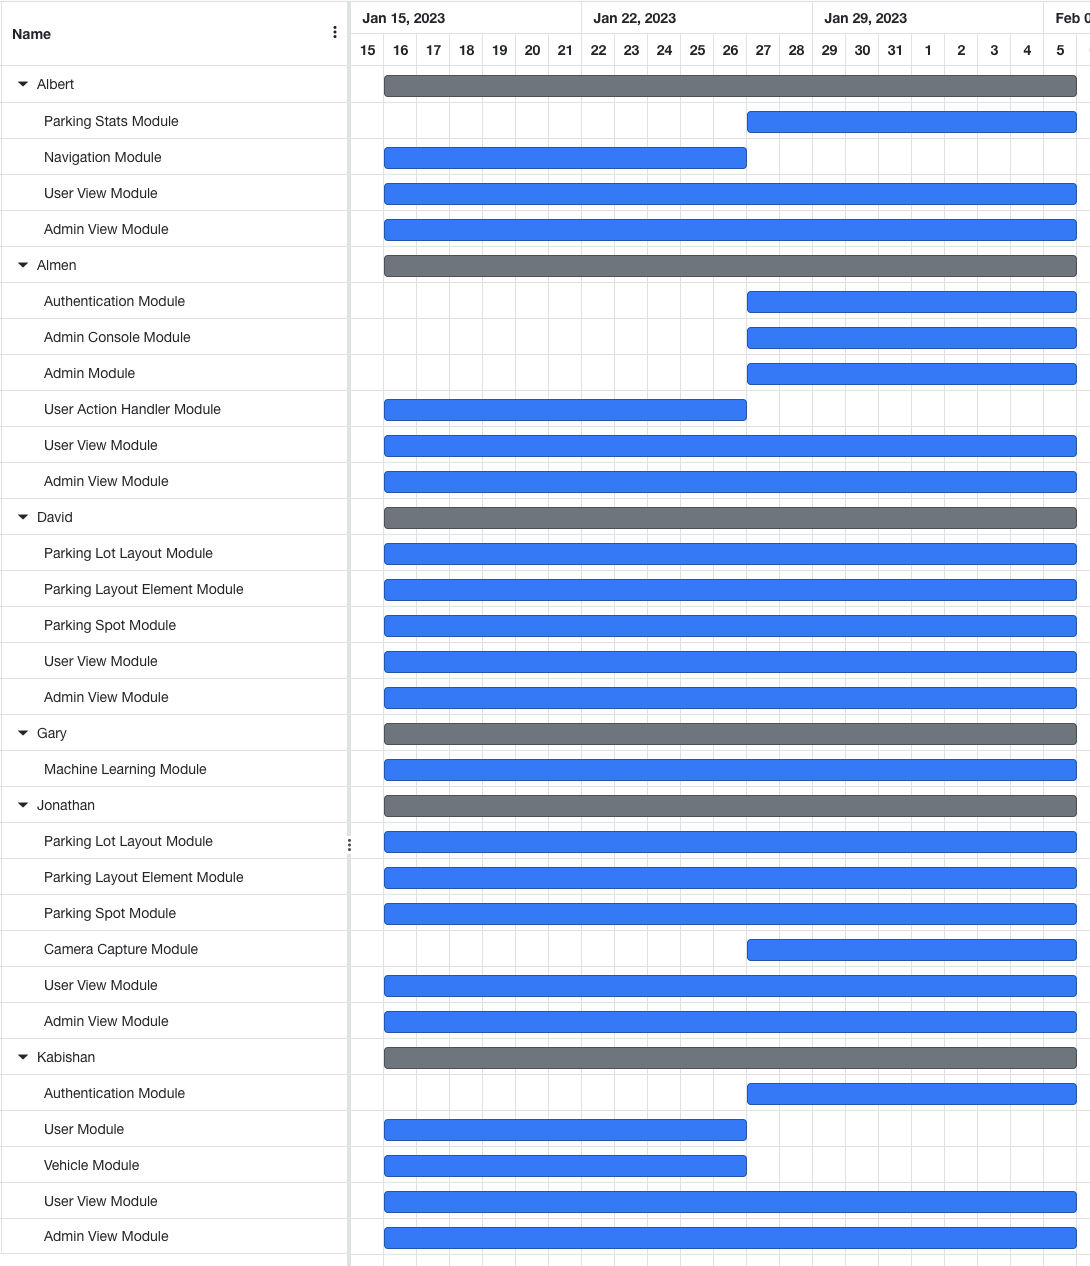
\includegraphics[scale=0.6]{timeline.png}
        \caption{Timeline}
        \label{fig:timeline}
    \end{center}
\end{figure}

% \bibliographystyle {plainnat} \bibliography{../../../refs/References}

\newpage{}

\appendix
\section{Interface}

\begin{figure}[hp!]
\begin{center}
    \fbox{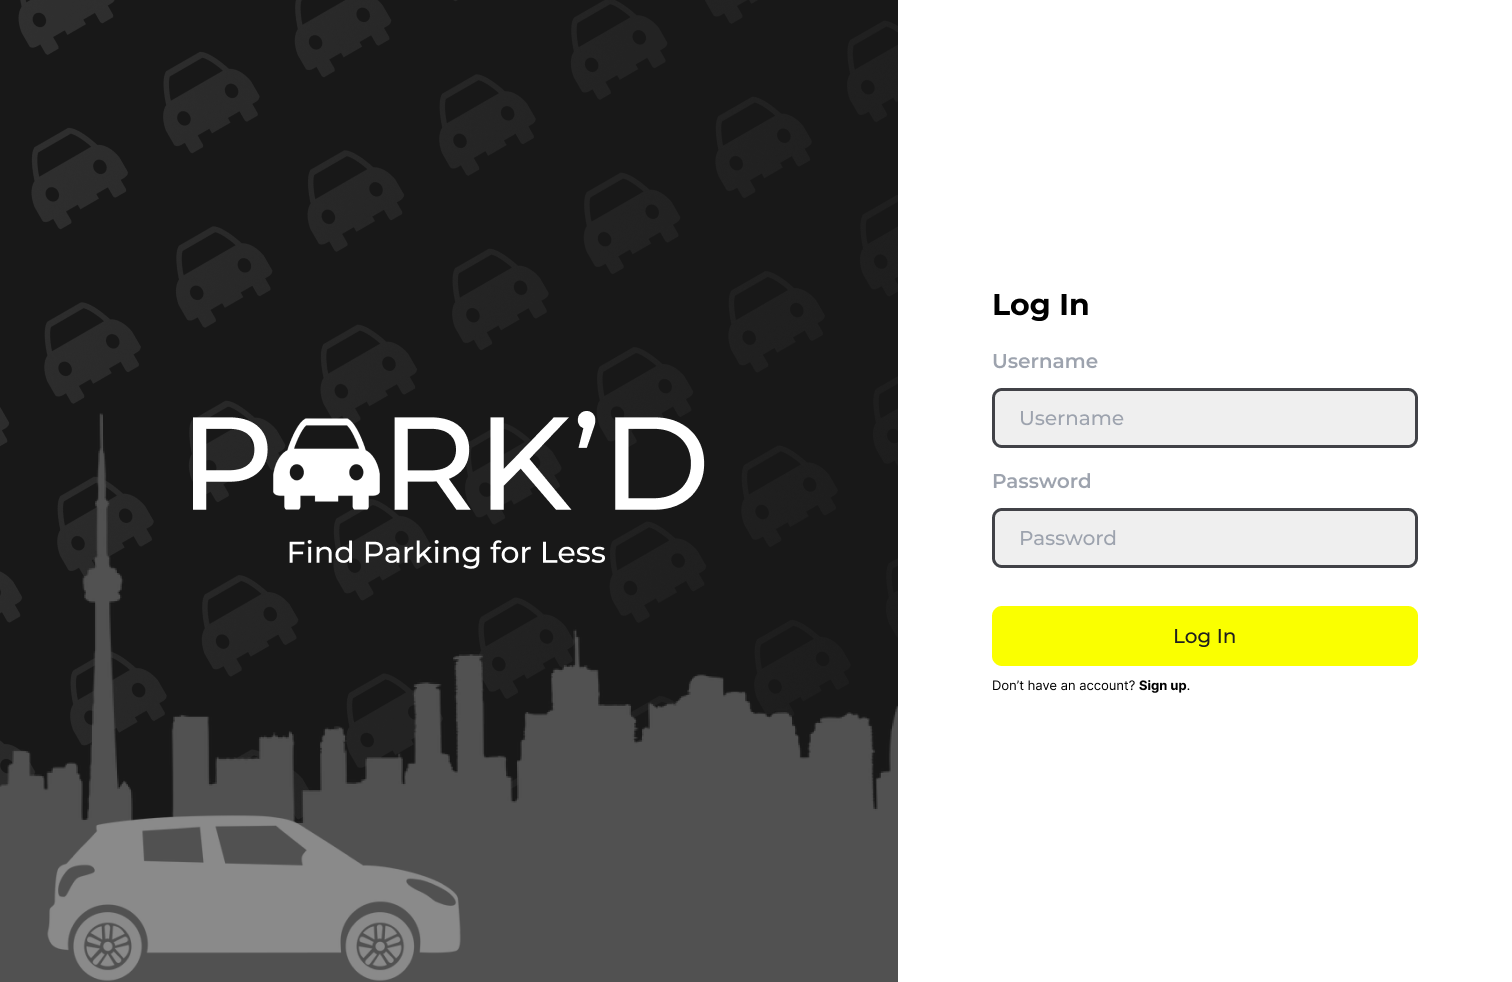
\includegraphics[scale=0.3]{Login Screen.png}}
    \caption{Login Screen}
    \label{fig:login}
    \end{center}
\end{figure}

\begin{figure}[hp!]
\begin{center}
    \fbox{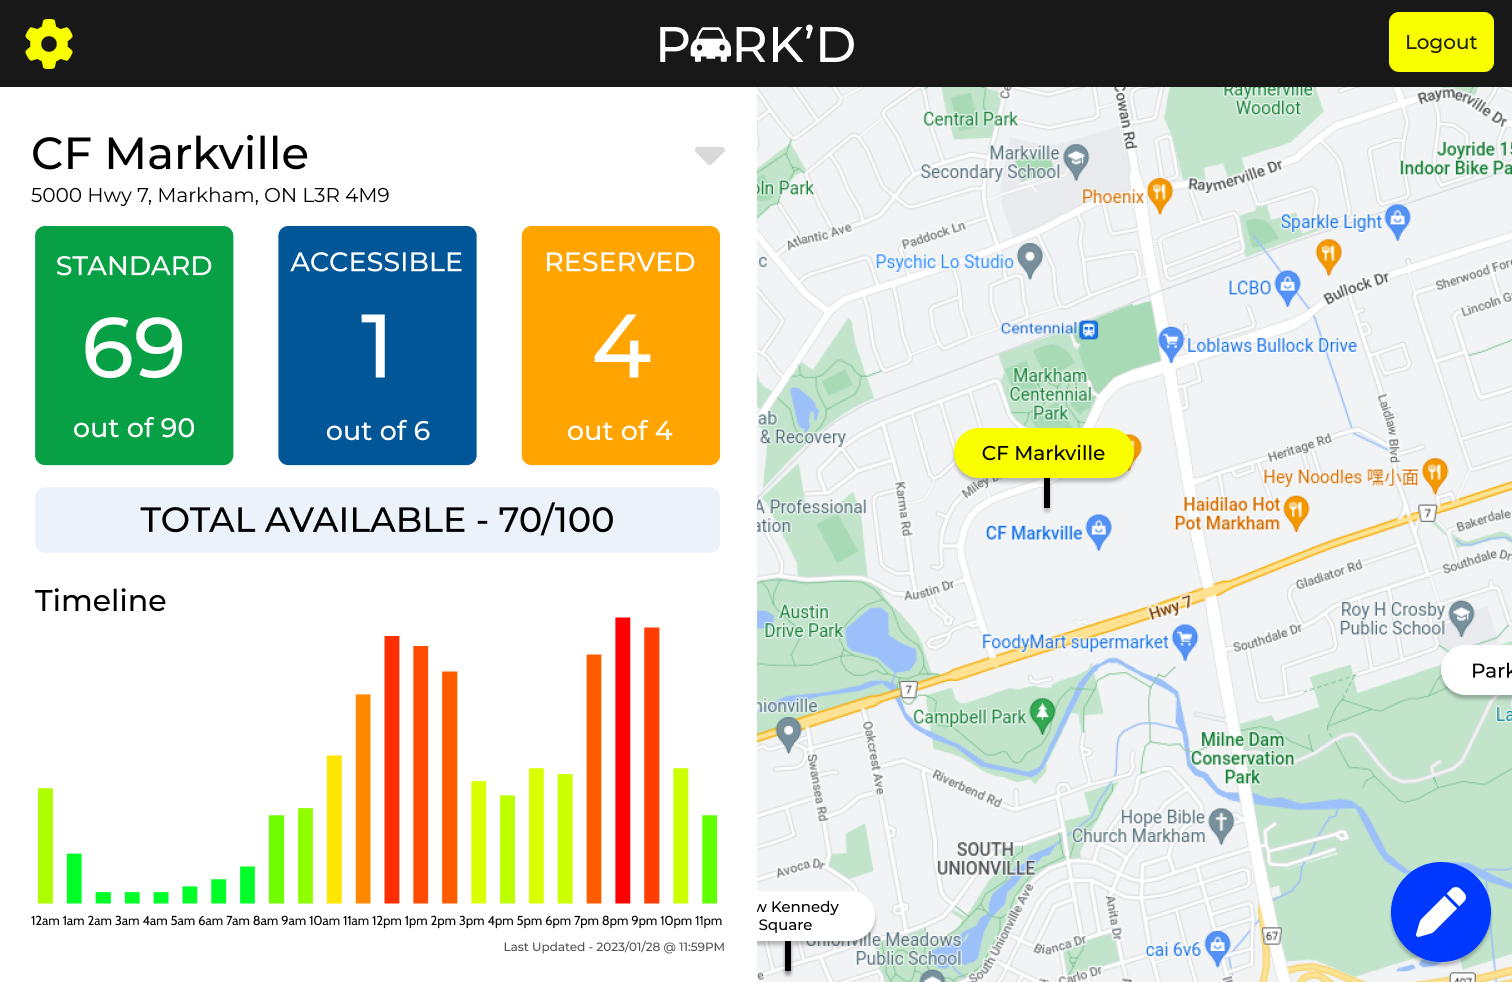
\includegraphics[scale=0.3]{Analytics.png}}
    \caption{Admin View - Analytics Screen}
    \label{fig:analytics}
    \end{center}
\end{figure}

\begin{figure}[hp!]
\begin{center}
    \fbox{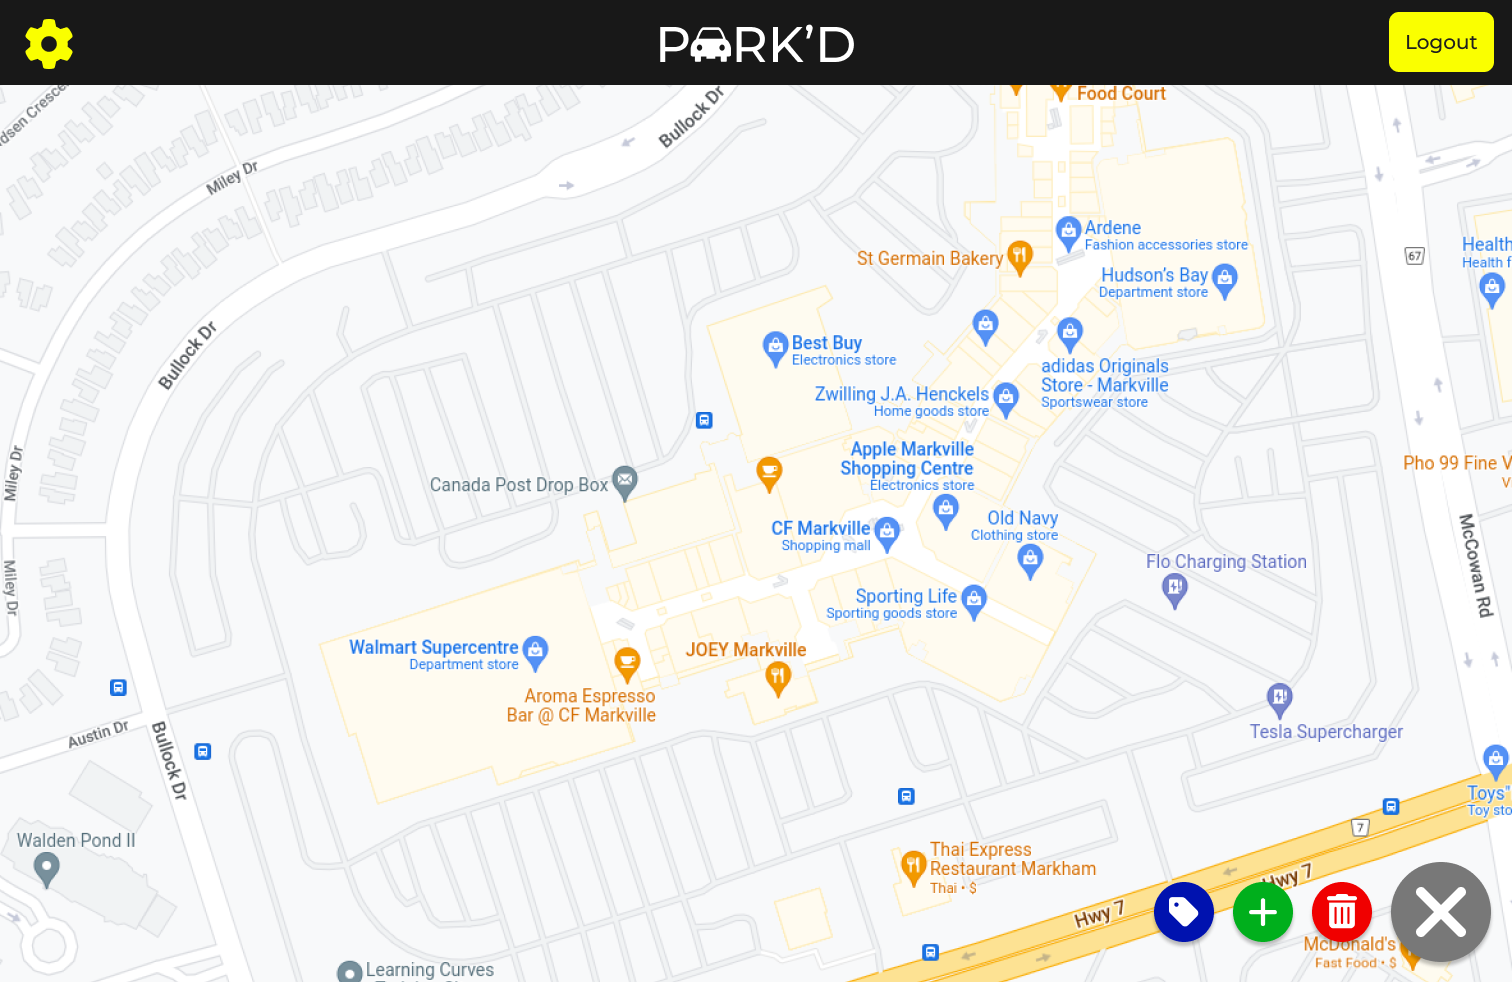
\includegraphics[scale=0.3]{Edit.png}}
    \caption{Admin View - Edit Screen}
    \label{fig:edit}
    \end{center}
\end{figure}

\begin{figure}[hp!]
\begin{center}
    \fbox{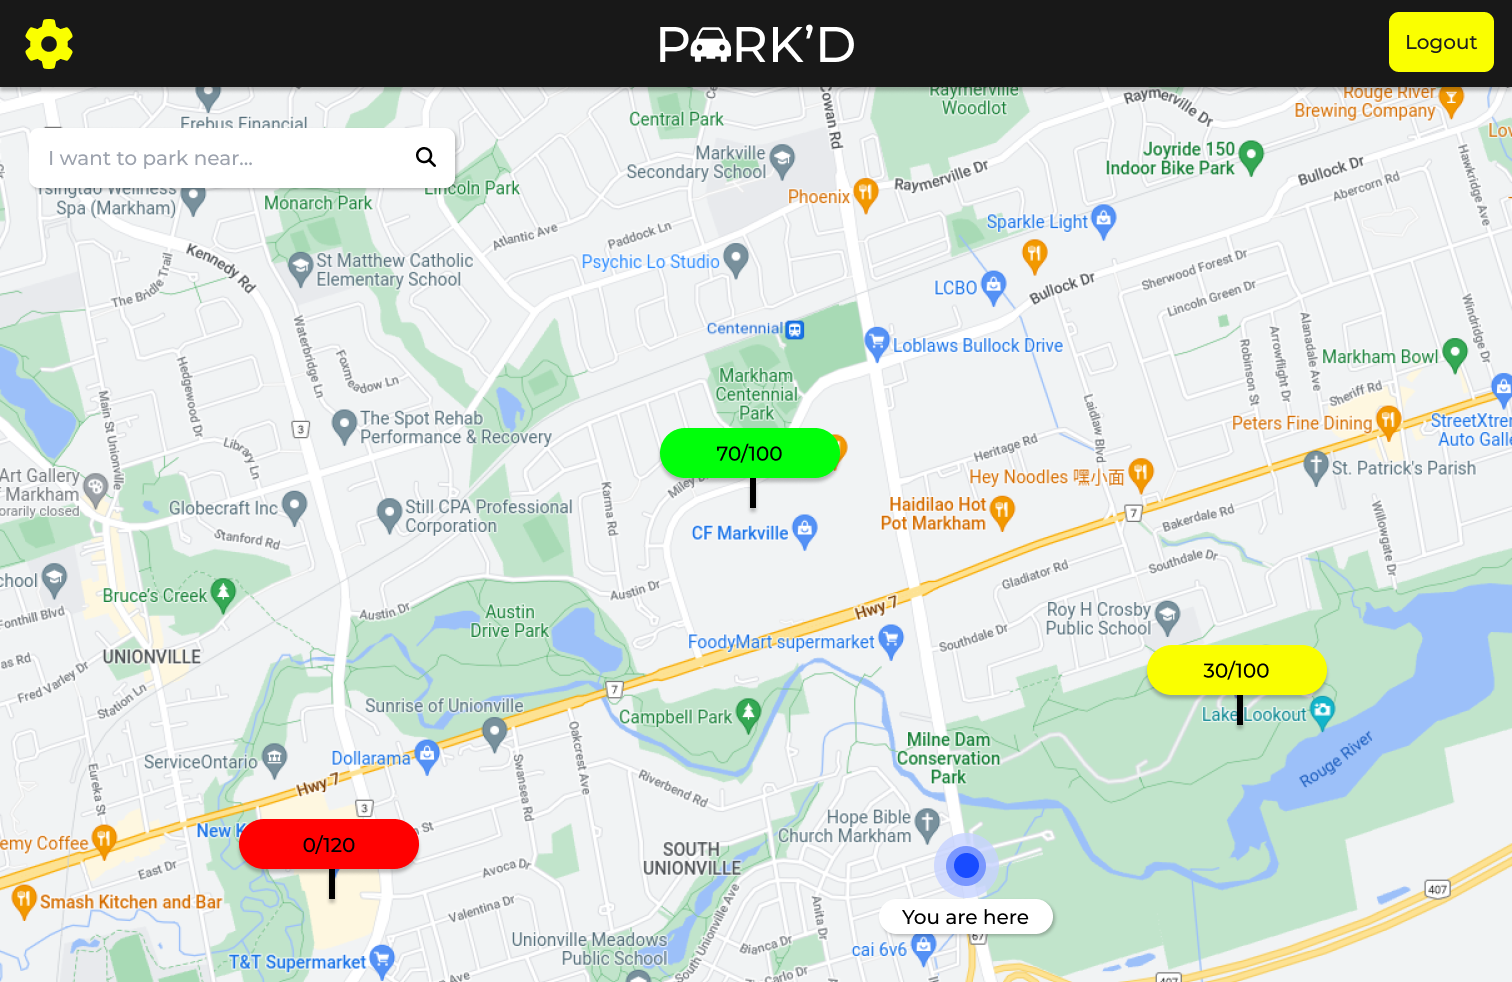
\includegraphics[scale=0.3]{You Are Here.png}}
    \caption{User View - You Are Here}
    \label{fig:youarehere}
    \end{center}
\end{figure}

\begin{figure}[hp!]
\begin{center}
    \fbox{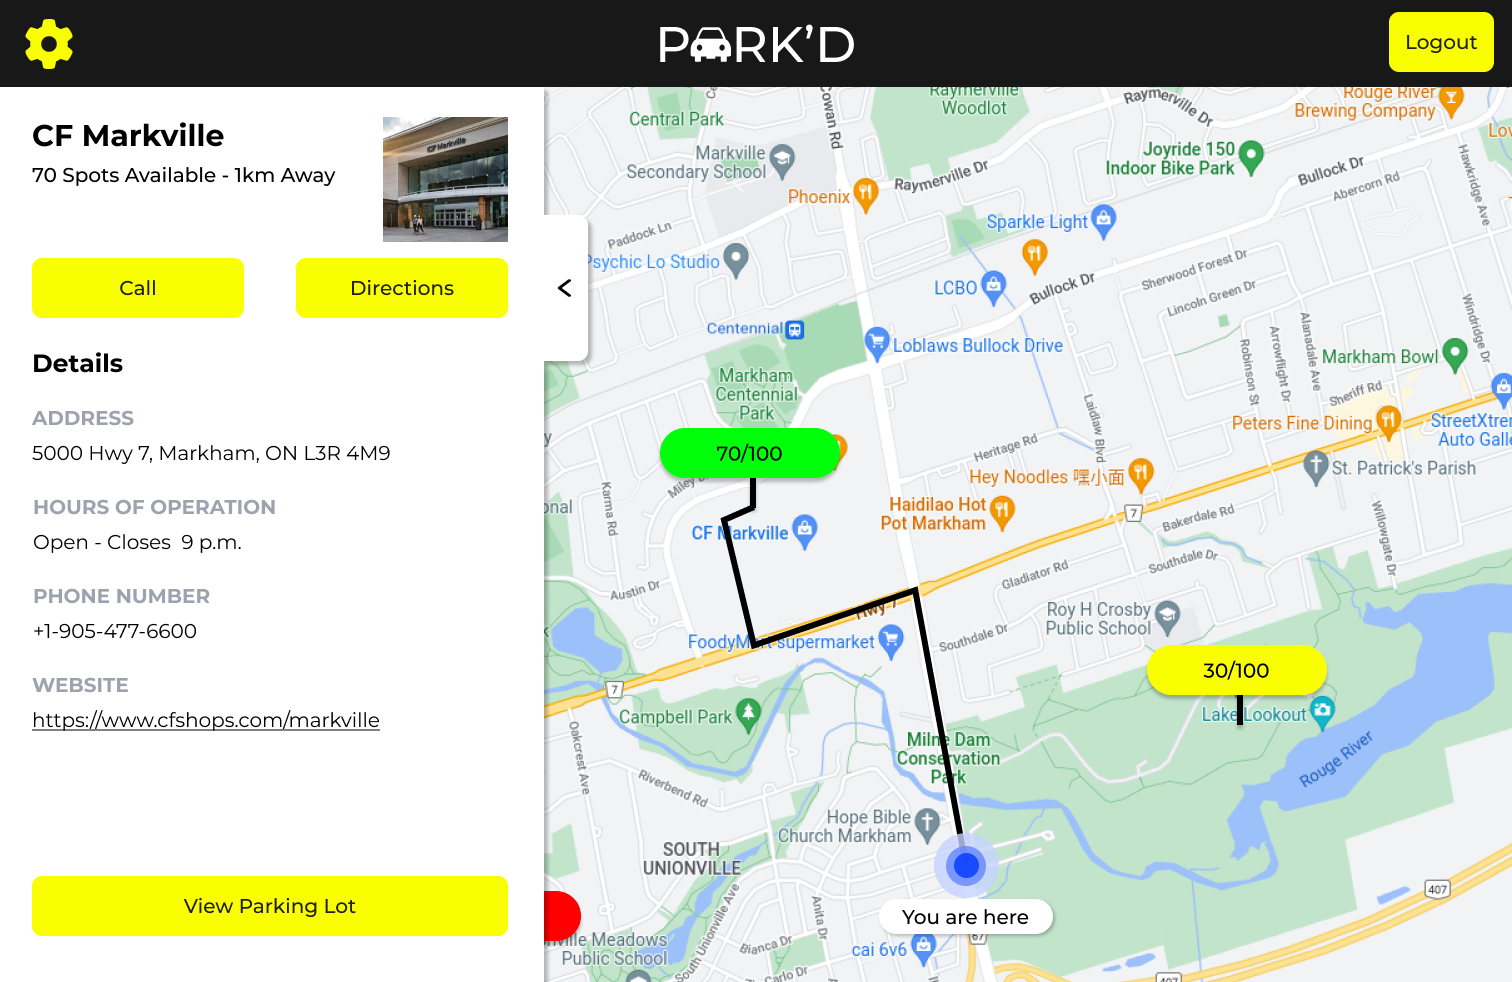
\includegraphics[scale=0.3]{Description.png}}
    \caption{User View - Description Screen}
    \label{fig:description}
    \end{center}
\end{figure}

\begin{figure}[hp!]
\begin{center}
    \fbox{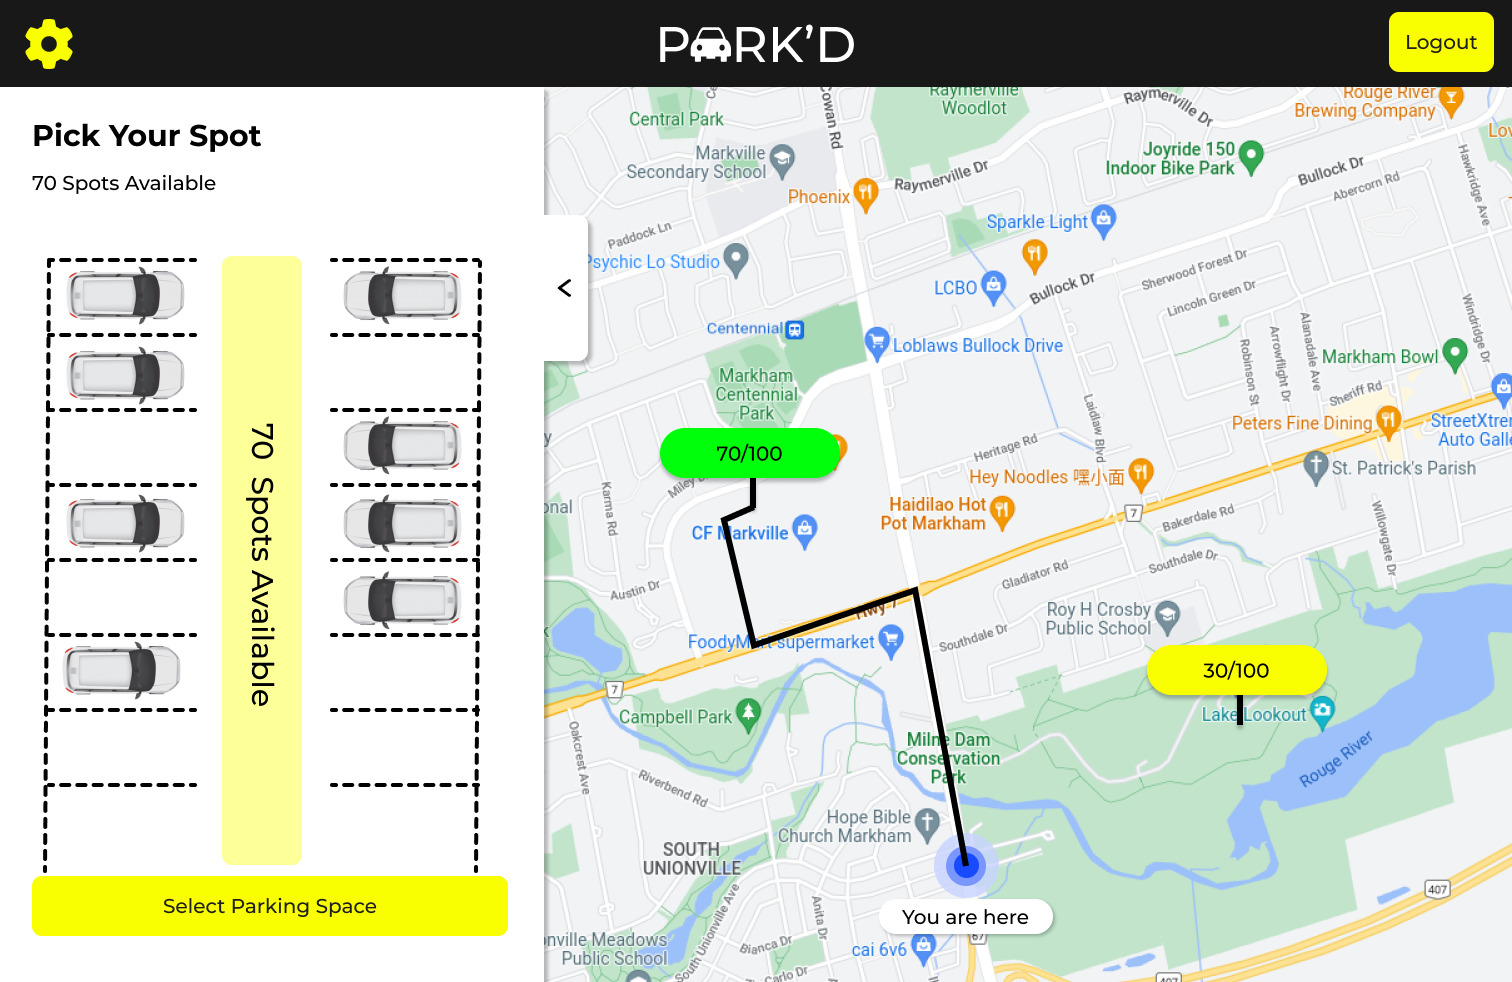
\includegraphics[scale=0.3]{Pick Your Spot.png}}
    \caption{User View - Pick Your Spot Screen}
    \label{fig:pickspot}
    \end{center}
\end{figure}

\begin{figure}[hp!]
\begin{center}
    \fbox{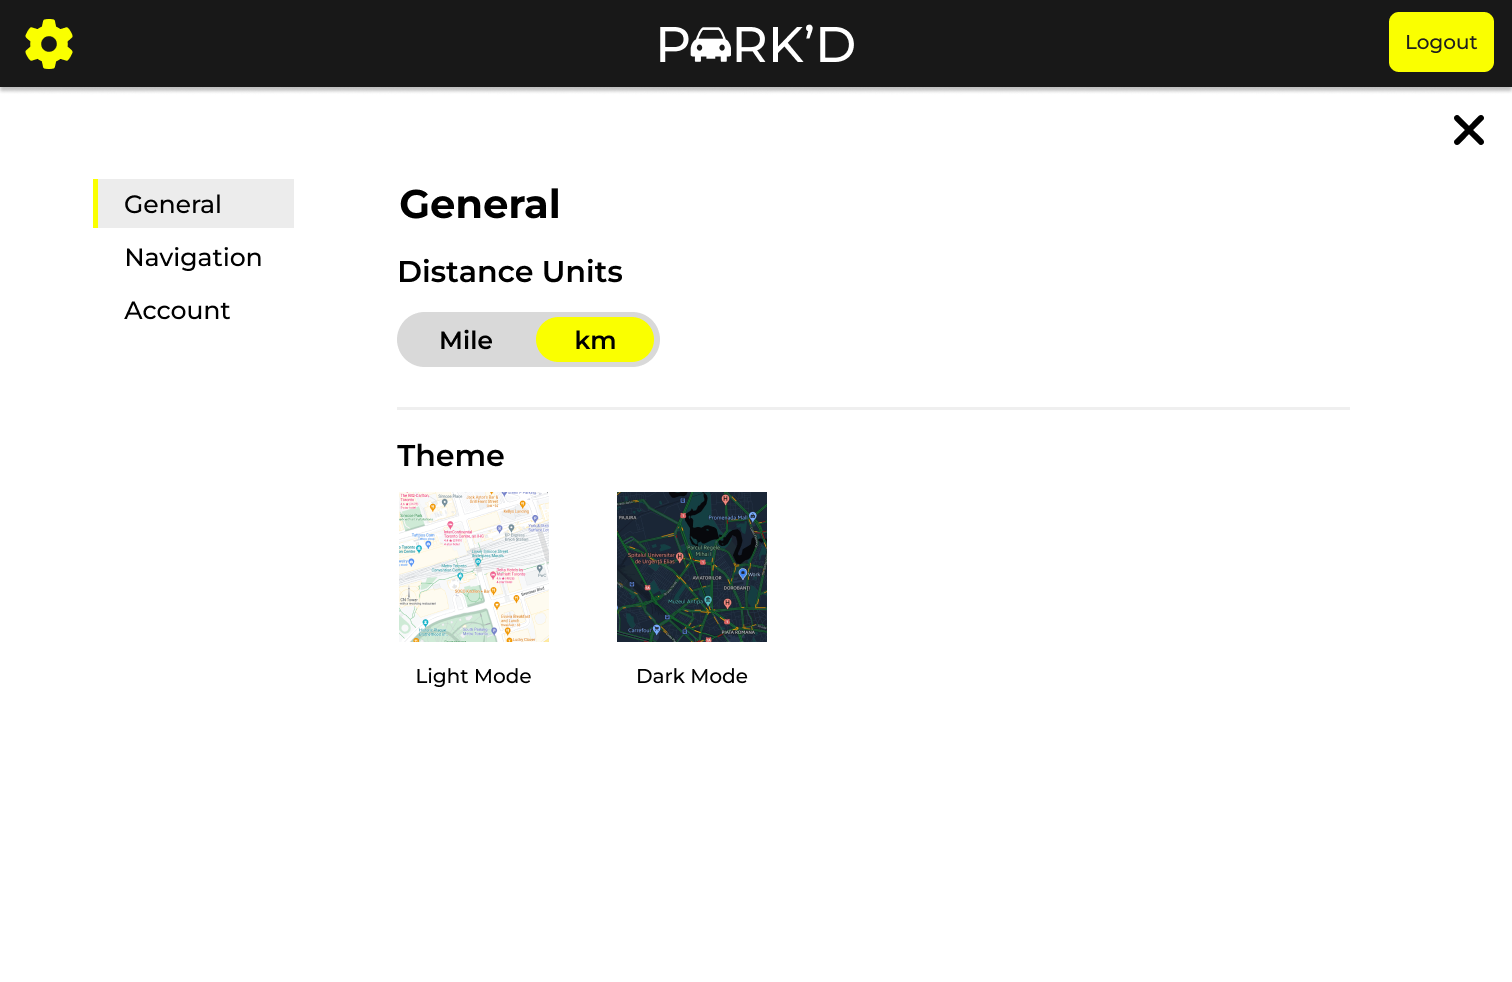
\includegraphics[scale=0.3]{Menu - General.png}}
    \caption{User View - General Settings Screen}
    \label{fig:settings}
    \end{center}
\end{figure}

\newpage 
\section{Mechanical Hardware}
N/A
\section{Electrical Components}
N/A
\section{Communication Protocols}
N/A
\section{Reflection}

The information in this section will be used to evaluate the team members on the
graduate attribute of Problem Analysis and Design.  Please answer the following
questions:

\begin{enumerate}
  \item What are the limitations of your solution?  Put another way, given
  unlimited resources, what could you do to make the project better?
  (LO\_ProbSolutions)
  
  \begin{enumerate}
  \item Our navigation system is simple and intended only to get the user within
  the general vicinity of their parking space, with the assumption that they
  will be able to locate it from there. The plan is to use a pre-existing
  mapping API, which for most parking lots will only map the main lanes. Given
  additional resources it may be possible to implement a more granular
  navigation, akin to those used in malls to locate specific stores, for
  example.
  
  \item The current solution for determining the layout of a parking lot relies
  on an administrator to specify relative locations for each space. The back-end
  model is only intended to poll spaces for their current status, not to
  determine where those spaces are located. Extra time and resources could allow
  for a more complex model capable of returning such information to be directly
  displayed by the front-end.

  \item Due to our solution's reliance on overhead cameras and clear aerial
  visibility, the user interface will not function with enclosed parking
  garages, or parking areas with multiple levels. Spaces are displayed to the
  user on a two-dimensional plane, so there is no way to switch between
  different levels for spaces that are stacked on top of one another. Additional
  resources could be allocated to a custom-built view to support such
  situations.

  \item With the current solution, our navigation system does not offer
  appropriate accessibility features such as voice commands/prompts and minimal
  number of taps to perform an action. Currently, once selections are made,
  minimal further interaction is needed, but additional resources could be
  allocated to user interface improvements to make hands-free operation as easy
  as possible.

  \end{enumerate}
  
  \item Give a brief overview of other design solutions you considered.  What
  are the benefits and tradeoffs of those other designs compared with the chosen
  design?  From all the potential options, why did you select documented design?
  (LO\_Explores)
  
  \begin{enumerate}
  \item The use of GPS, rather than overhead cameras, was considered to map
  parking lot layouts and mark occupied spaces. By noting at what specific
  coordinates app users tended to park their cars, the idea was to crowd-source
  the layout of a given parking lot over time. Spaces would be marked as
  occupied if an app user's vehicle was parked at the given coordinates. This
  would eliminate the need for cameras, as well as manually creating a layout.

  There are two main issues. First, the application would need to see broad
  adoption for it to be useful. Many users would be needed for an entire parking
  lot to be mapped out in an acceptable time frame, and then spaces would only
  be marked full if occupied by an app user. Second, mobile GPS varies widely in
  its accuracy, and is often not precise enough to determine exactly which
  parking spot has been occupied.

  \item We considered the possibility of installing hardware on each parking
  space responsible for polling the state of its space and reporting back to a
  central system. Using specifically designed hardware would eliminate the
  issues stemming from variations in camera quality and position, or GPS
  accuracy.

  The issue with this idea is the difficulty of scaling up over large or
  multiple parking lots. Enough hardware would be needed for every parking
  space, and the hardware would need to be installed manually for every space.
  \end{enumerate}
  We selected the documented design as it needs very little from the end user in
  comparison to other candidates. It relies solely on separate camera hardware,
  and not GPS or specialized hardware. It is intended to work just as well
  regardless of the number of people using the application, and without the need
  for extensive hardware installation.
\end{enumerate}

\end{document}